\chapter{Toolchain} \label{chap:toolchain}

The overall idea on how to achieve a toolchain that fully supports the requirements described in section \ref{sec:vision_for_a_dsl} and to supports the modeler in the modeling process is, to develop an integrated development environment like they are used in computer sciences and software development. IDE’s, such as the well known Eclipse IDE, Netbeans or MS Visual Studio  are very common and crucial tools in the area of software development. They provide the software developer with a set of very useful tools and functionality such as code completion, syntax highlighting, debugging features and so on. All of these tools allow the software developer to manage much more complex software projects and increases its productivity. Based on the premiss that software developers are nothing else than “modeler of source code”, the similarity to the problems in the environmental modeling domain are obvious. This chapter tries to outline the idea of such a specialized IDE for environmental modeling. In order to do this, we decided to describe a workflow including the steps a modeller has to take, to define a model with such an IDE.
\begin{figure}[h]
	\centering
	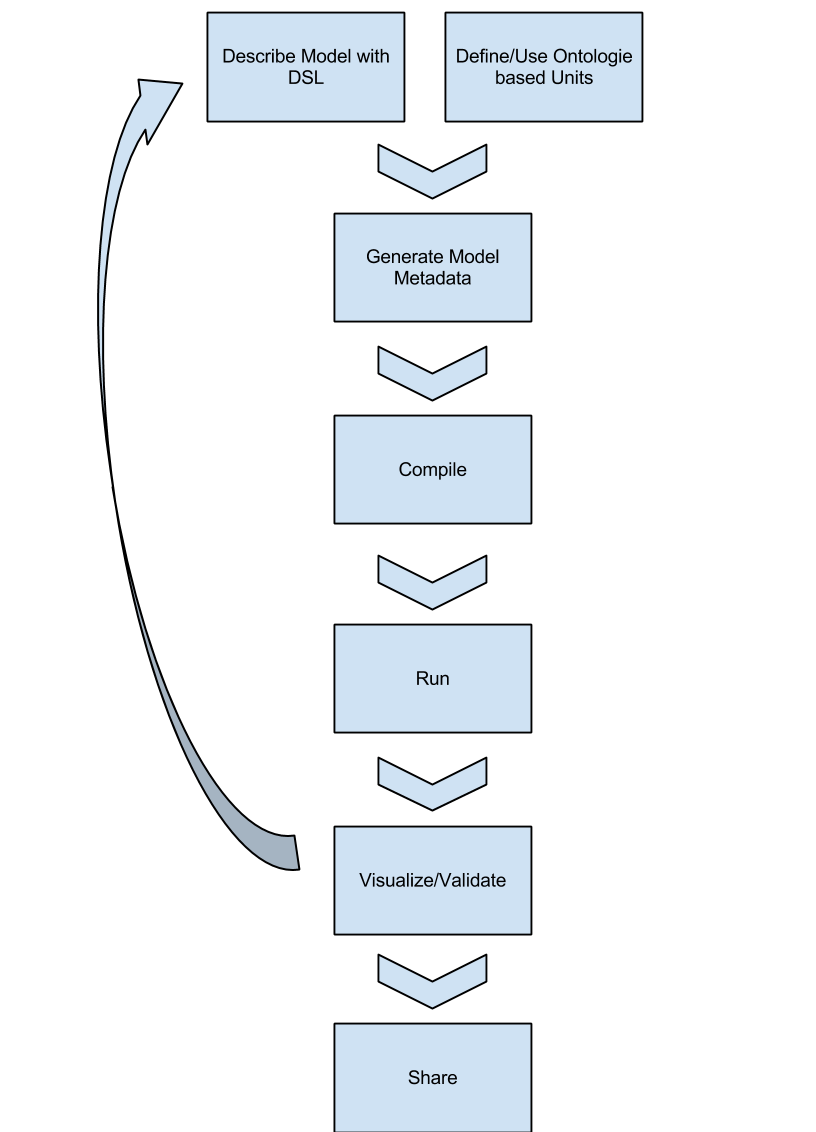
\includegraphics[width=0.7\textwidth]{pics/toolchain/modeling_workflow.png}
	\caption{modeling workflow \label{fig:modeling_workflow}	}
\end{figure}

A very extensive discussion of a modeling process can be found in \autocite{Jakeman2006602}. Hence this article targets the quality of the model process itself and does not take into account how this workflow can be supported by tools, we decided to take a much more simpler modelling workflow that is more suitable and based on the steps necessary using an IDE for the modelling process.Picture \ref{fig:modeling_workflow} depicts this simplified modeling workflow.


We decided to start with the implementation of the model. Prior steps such as defining the model purpose, specifying model context and so on, like they are recommended in \autocite{Jakeman2006602} are left out intentionally in fact we want to emphasize the use of the IDE and to concentrate on the requirements derived from chapter \ref{sec:vision_for_a_dsl}. In the following sections we want to explain the different steps and what features the IDE can offer to support the user in more detail. 

\begin{figure}[h]
	\centering
	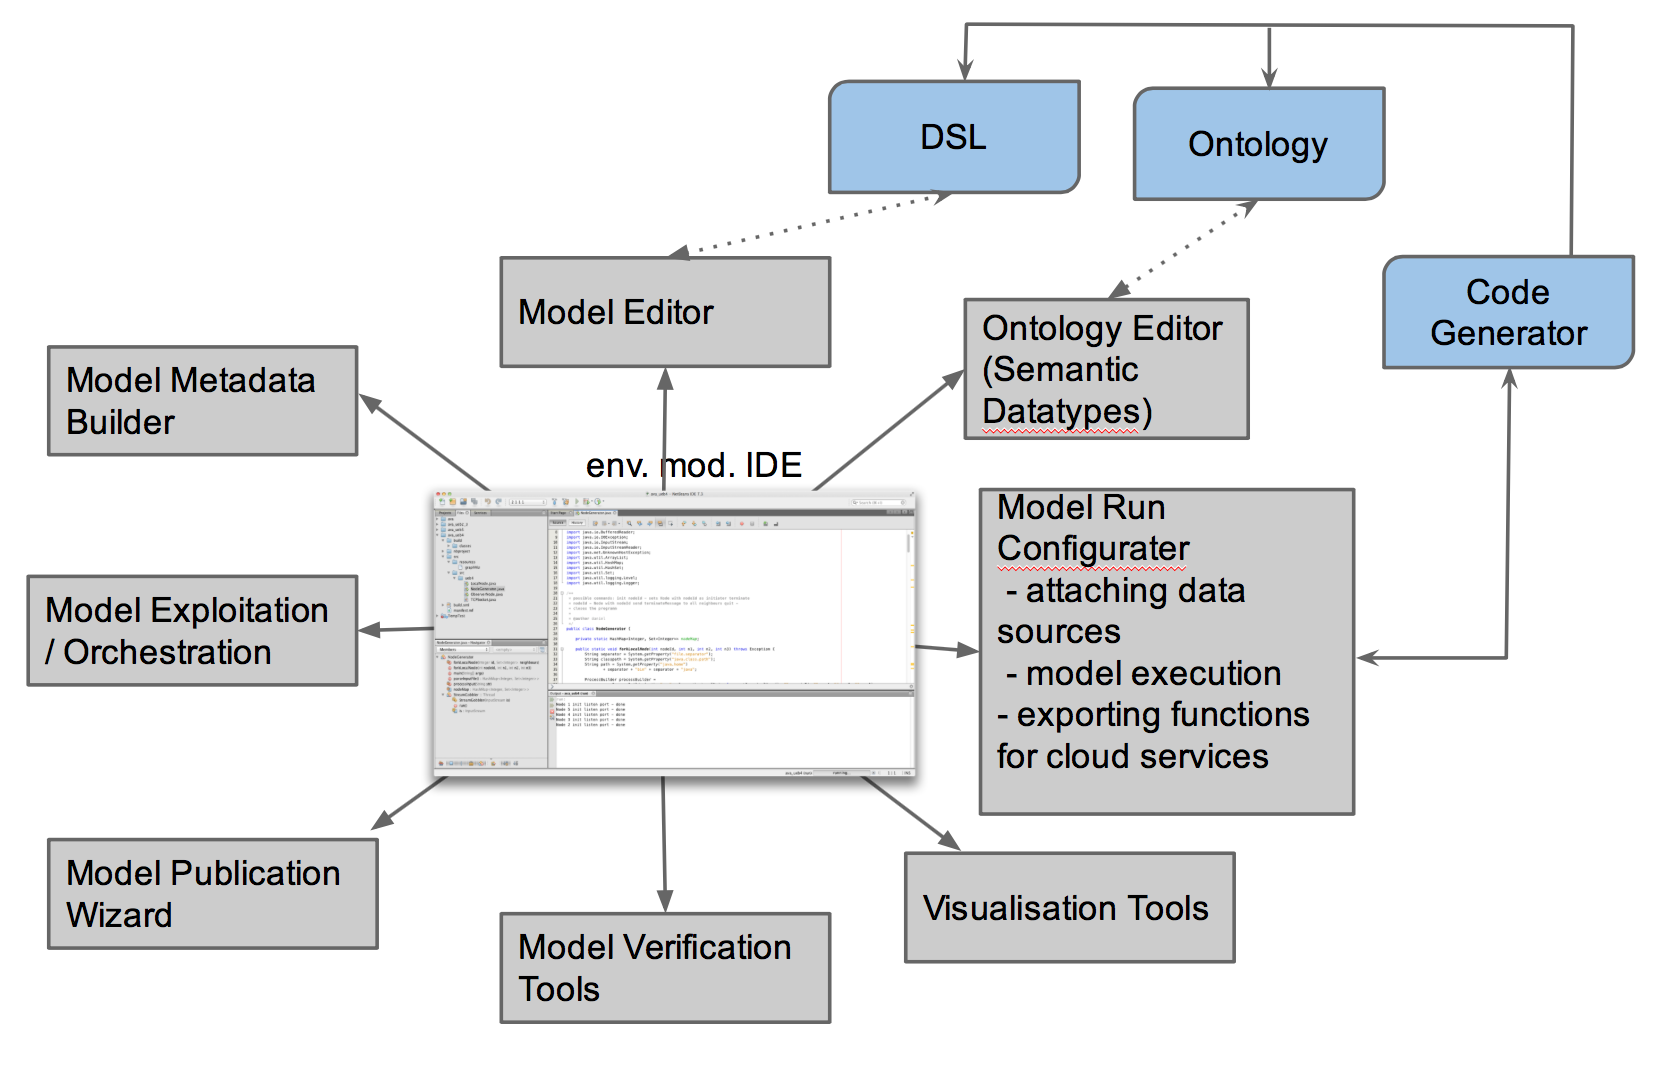
\includegraphics[width=0.99\textwidth]{pics/toolchain/toolchain.png}
	\caption{modeling workflow \label{fig:toolchain}}	
\end{figure}


\section{Writing a model} \label{sec:writing_a_model}
The modeler starts with the implementation/coding of the model. Since this is the most basic part of the IDE and the main interface for the user, this is the place to include the most relevant and crucial tools to support the user during the coding phase. These features are very diverse and range from very simple and basic ones like code completion, syntax highlighting, automatic warnings and action items to much more complex and specialized ones that belongs to the requirements from chapter \ref{sec:vision_for_a_dsl}. One of these very specific features are domain specific semantic datatypes and the handling of typical operations as explained earlier. In order to achieve these features, it is necessary to define important semantical aspects of entities and datatypes used in the model.


A very common approach to define the semantics in a formal and machine readable way (which is important for later code generation) are ontologies\footnote{see \nameref{sec:app:ontology} in the appendix for a short explanation of ontologies}. The reasons for this are discussed in \autocite{toolchain:protege_onto}, \autocite{toolchain:gruber} and \autocite{toolchain:musen}. And also in the environmental domain ontologies are often used and are a very common way to define semantics of entities. \autocite{dsl:muetzelfeldt}, \autocite{Villa2009577}


Therefore the semantics of every used entity or datatype must be defined in an ontology which then can be used to automatically check consistency of the model, and that allows the IDE to handle typical operations like automatic unit conversions. Actually there are a set of projects that has focused on this topic  and that developed a set of ontologies that define the semantic of entities in the environmental domain.  QUDT, which stands for Quantities, Units, Dimensions and Data Types in OWL and XML \autocite{toolchain:qudt} is one of these projects and one of it’s goals is to ``to provide a unified model of, measurable quantities, units for measuring different kinds of quantities, the numerical values of quantities in different units of measure and the data structures and data types used to store and manipulate these objects in software'' \autocite{toolchain:qudt}. Another, more famous project is Nasa SWEET (Semantic Web for Earth and Environment Technologies) \autocite{toolchain:nasa_sweet} which provides a very extensive set of ontologies and ``include several thousand terms, spanning a broad extent of earth system science and related concepts''\autocite{nasa_sweet_guide}.


Although these projects describe a huge set of environmental concepts it is conceivable that a modeler needs additional semantical aspects of an already existing concept or to create a totally new entity that isn’t already semantically described in the used ontology set. Therefore the user must have the possibility to edit the underlying ontologies.  There are already good tools that allow the creation of ontologies. Protege \autocite{dsl:protege} is a very common tool for this. Although it would be sufficient to provide the user access to the underlying ontologies and thereby giving  the possibility to edit them with standard tools we think that providing the user with a specialized tool to do this is a much more better idea.


The two main reasons for this are simple. It is not clear if every user has the necessary knowledge to work with an ontology editor like Protege or has a fundamental knowledge of ontologies itself. This lack of experience and knowledge could be a very difficult to overcome hurdle for these users and therefore should be avoided. Another more important reason to hide the complexity of the ontology is that it has a very specific design and probably a very large extent. Providing the user full access to the ontology, it could easily happen that changes of  the user leads to inconsistencies accidentally. Providing the user a special tool that allows him to import his semantic datatype descriptions would avoid these disadvantages totally and can lead to a better acceptability. 


Furthermore such a tool could be much better integrated in the modeling workflow. If the user defines a new entity in the DSL, the IDE could check automatically if the ontology contains semantical descriptions of this entity. If not it could trigger the user to define such semantical descriptions by starting the available tool. Another possibility to react on this situation is to show warning messages or an action tag, that reminds the user to define the semantics later on.

\section{Generating model metadata}

Another important task the user wants to do with his new developed model, is to prepare it for a later reuse by other modelers or a later reuse by himself. This makes it necessary to add a set of rich metadata to the model that describe the model itself and simplifies the reuse of it. Furthermore if a model provides such metadata in a standardized, formal and machine readable way it also should be possible to generate a kind of modellibrary or, to think one step further, to automatically composite different models like it is done with web services and the BPMN or BPEL languages. Some ideas how to achieve this are discussed in more detail in the step sharing a model.


The first question is what kind of metadata must a model provide to allow such a further machine based processing, how can it be integrated in the IDE and how can the user control necessary details of the process of meta descriptions.
Although this is a really important step conceptually, we think that the occurring problems are not difficult to solve from a technical point of view. Hence the underlying problem of describing entities with metadata had occurred also in other domains than in environmental modelling and are solved there already, thus we think that it must be possible to adapt these solutions.
One example, which is very similar to the one described above, is the service oriented architecture (SOA) principle. In this paradigm, software components are provided as (web) service. The service functionality, its input parameters and the output parameters are described in standardized and formal way. In terms of SOA this is mostly done with the Web Service Description Language. If we suppose, that the written environmental models are nothing else than a kind of service or software component, it is obvious that it must be possible to provide meta information of an environmental model. This answers also the question what metadata must be provided by the model. The model itself can be thought of as a black box, which needs some input parameters, makes some calculations based on this input, and returns the processed results. The following list depicts some meta information that are needed following the WSDL approach. \autocite{dsl:muetzelfeldt}

\begin{enumerate}
\item input parameters
\item output
\item formats
\item used constants
\item run specifications
\item user defined metadata
\end{enumerate}


Besides that rough and overlooking argumentation, there are some existing modeling environments that make use of a very similar concept. Muetzfeld et. al describes in \autocite{dsl:muetzelfeldt} the idea of declarative modeling. The idea there is to describe the whole model in a declarative manner and hence abstract it from the concrete implementation. In order of doing this modeling environments like Simile (see chapter \nameref{sec:similie}), ACSL, Stella, Modelmaker, Powersim or Vensim ``enable a model to be saved to file as a design specification'' \autocite[32]{dsl:muetzelfeldt} which also means that metadata of the model can be described.


Another example of the environmental domain, which also topics the description of models through metadata is OpenMI. OpenMI stands for Open Modelling Interface and Environment and its originally purpose is``[...]to facilitate the linking of models.'' \autocite[70]{adgeo-4-69-2005}. In order to do this OpenMI provides a set of standard interfaces that describe model parameters and so on.


Besides the feasibility of this issue, another question is how the user can generate the necessary metadata for his model. A good example for doing this in the software domain, is JavaDoc. JavaDoc is a tool that allows the Java programmer to automatically generate documentation of his program based on annotations he integrates directly to the source code. The documentation itself is then presented in HTML. This approach has some good key concepts. The first one is that the user can easily provide the necessary meta information through annotations directly where they are needed. Furthermore it separates the final representation from the information itself. To give an example from the environmental domain, OMS also uses annotations to provide metadata of the models. According to David et al. they defined a “annotation standard” for the following features: “(i) simplifying component integration, (ii) implicit autoscaling of simulation models in multicore and multiprocessor environments, (iii) providing for modeling simulation traceability and integrity, and (iv) autodocumentation of models and simulations'' \autocite[2]{dsl:oms-handbook}.


We think that it is a good idea to transfer the ideas of JavaDoc/OMS to the toolchain of our environmental modelling IDE. This means that the DSL must provide the possibility to annotate the single entities. Furthermore a tool that generates a model  description (may be based on OpenMi) based on these annotations must be developed.


An alternative approach could be to provide the user a GUI-based tool to gather and edit the meta information. Again, this solution would need a kind of generator that generates a model description based on the metadata.


To complete this discussion, we want to call attention to another very important issue. The description of a model and its metadata and all the possibilities it provides are only achievable if the generated description is popular and widely spread. This means that the description must come up to a common standard. To our knowledge such a standard does not exists.


To put it in a nutshell, we think that this step is more a question of how to integrate the feature in a user friendly way and we do not see problems in the technical feasibility.

\section{Run and verifiy}
Once the model is written within the IDE it must be possible to run the model as simple as possible and get all necessaries simulation results the user requires. To run the model it is necessary to attach some datasources, because the data is not part of the model \autocite{dsl:muetzelfeldt}. This task does not rely to the concrete modelprocess. It must be possible to attach and detach datasources in a simple way.(see also \ref{sec:vision_for_a_dsl})


The model itselfs would define dataslots on which data sources can be attached. In chapter Second DSL Draft the describe statement is used to describe a mapping beetwen one datatupel to another, like an mathematical funktion. Further these statemant can be used as dataslot. In this way the belonging value is not mappend with an formula. In chapter \ref{sec:second_dsl_draft} the describe statement is used to define a mapping between a input datatupel and output datatupel. These mapping is done with a mathematical formula. Further the describe statement can be used as a dataslot. Used in this way the describe statements provide the modeller the possibility to connect to another model or database which will handle the mapping between input and output data. Further the model metadata describes the structure of the input data which is expected. Based on these informations it is possible that the IDE generates an adapter from the available data sources to the model \autocite[81]{Villa2009577}. This process would be entirely transparent for the user. The user will just use a wizard dialog to plug all available data sources to the model using the drag and drop metaphor. All data sources which can not converted to a format the model expects, would automatically marked as inappropriate. If one source, which the user wants to use is marked as inappropriate, he has to reconsider the model definition.


Another use case which requires a simple possible way to attach datasources is the calibration of the model. That means that data is used on which the results are already known. For example to verify a weather forecast model some old weatherdata would be plugged into the model and the model would be eventually run. The results of the simulations would be compared to the real weather events which happens in the past. The difference between the simulation results and the reality is the precision of the model. But this precision only relies on the specific simulation, it is possible that a simulation with other data belongs to an other precision. To approximate an absolute model precision it is necessary to run such a simulation multiple times with various data. This can be a painful task so its necessary to provide a mechanism to facilitate this. The goal of the model calibration is to determine how to justify the parameter to improve the precision \autocite{toolchain:ems-model_calibration}. If there is enough data available it is imaginable to plugin the datasources and find the best parameter fitting automatically. A tool that already solve this problem is GMS \autocite{toolchain:gms_overview}. How these process looks like in GMS is described in \autocite{toolchain:ems_pram_estimation}.


The main function of the IDE aiming to run a model is to display the results of the simulation. Running the model means that the code generator generates the code which will be compiled and eventually executed. The IDE is able to choose the right presentation format e.g. the diagram type or a specific datatable format. These decision can be done on basis of the metadata which specifies the model output data. Of course it is possible to choose a format by your own.


In \ref{sec:vision_for_a_dsl}, it is described that the models and the calculation should be transparent and defensible. That requirement could be solved by logging all intermediate results. This logging can be consulted to debug the model. For these purposes a tool which allows the user the interactive exploration of the logged data is imaginable. For example the user can filter values of one specific variable for each simulation step, or he can filter a set of variables for one specific time step. Further the tool could be able to visualise the data with charts and graphs or can provide some statistical information. This would help the modeler exploring the logged data and can be used for debugging purposes.


Many models require a huge amount of computation power but some of these models can be written in a way which allows a parallel computation. Hence it seems to be conceivable that the IDE automatically recognizes if it is possible to distribute the calculation to multiple computers. These recognition would happen on basis of some keywords the DSL provides. Once the IDE knows that the computation is distributable the IDE can trigger the user to provide some additional information for the parallelization which can be for example credentials to a cloud provider. There is no need to use a specific Platform as a Service to deploy the model and run them in the cloud. The whole logic, which describes how the model is run on a virtual machine is known by the IDE. Hence the cloud provider must only provide a standardized infrastructure as a service. Because the vision of the DSL does not cover some distributed computation mechanisms these thoughts are not further proven.


\section{Sharing a model}

One of the main goals of the DSL and the toolchain is the ability to facilitate the reuse of all models. The greatest degree of reuse can be reached by sharing the models with an community of other modellers.


This possibility is reminiscent of the vision of webservices. On basis of the metadata it is possible to decide if the model fits into the needs of the modeller. The main benefit appears in the context of composing some models to an overall model. Here too, we can see the analogy to webservices (service composition).


One way to exploit to whole power of the metadescription could be to describe the interfaces of the required submodels and the IDE searches for suited models. In this point it is needed to extends the concepts which are used in webservices. To describe a webservice interface WSDL is used, but to achieve the vision of an automated submodel search, a ontology based description is required.


The biggest problem to achieve the vision of automated model search is to distribute the standard rather than the technical implementation.


Further, for this vision it is necessary to provide a central repository on which all modeller can register his models. To register the model on the repository the IDE provides a wizard to simplify these process. It is also possible to use a dialog to explore the repository by your own to find a suited model. In order to that huge mass of models, the IDE must provide some tools to filter the models. e.g. categorize or keyword search.
